Given
\begin{align}
	c_1 = \frac{7}{3},\,
c_2 = -6.
\end{align}
	From \eqref{eq:parallel_lines},
we need to find $c$ such that,
\begin{align}
	\abs{c-c_1} = \abs{c-c_2} \implies c = \frac{c_1+c_2}{2}
	 = -\frac{11}{6}.
\end{align}
Hence, the desired equation is
\begin{align}
	\myvec{3 & 2}\vec{x} &= -\frac{11}{6}
\end{align}
	See \figref{fig:chapters/11/10/4/21/1}.
\begin{figure}[H]
	\centering
	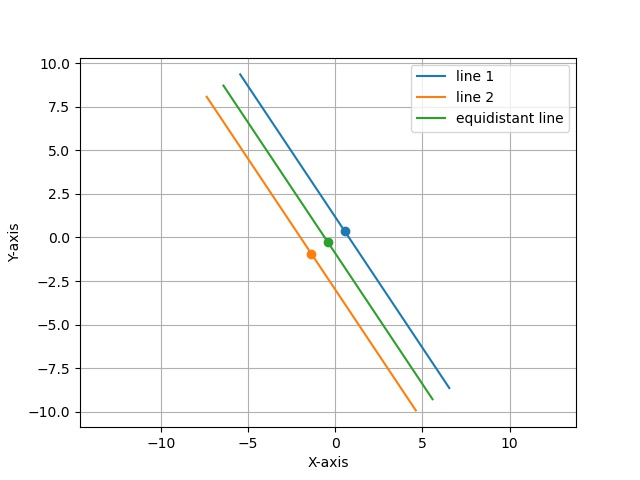
\includegraphics[width=0.75\columnwidth]{chapters/11/10/4/21/figs/line_plot.jpg}
	\caption{}
	\label{fig:chapters/11/10/4/21/1}
\end{figure}
